\chapter{Architektur}
Die Architektur unseres Projekts sieht an der Benutzeroberfl�che neben dem Navigations-Client einen Collector-Client und eine Admin-Oberfl�che vor. Im Hintergrund werden die Informationen in einer Datenbank gespeichert und mit Hilfe eines Webservice bereitgestellt.

\begin{figure}[H]
\centering
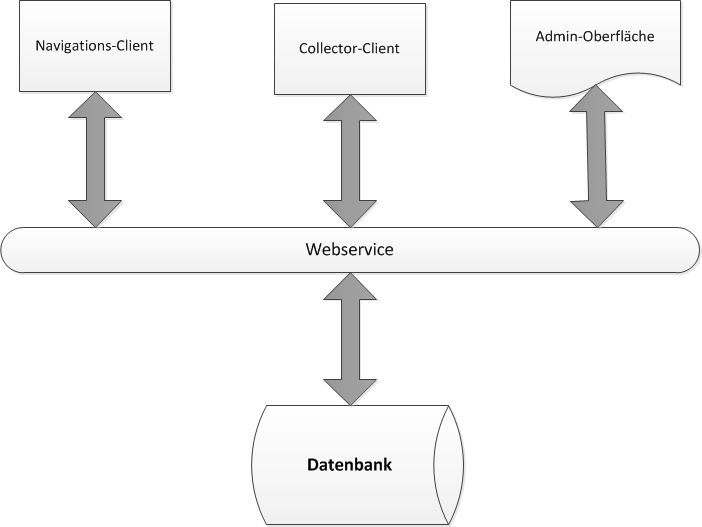
\includegraphics[width=\linewidth]{./Bilder/Architektur}
\caption{Grafische Darstellung der Architektur}
\label{fig:Achitektur}
\end{figure}

Der \textbf{Navigations-Client} ist die Bedienoberfl�che des Benutzers. Hier wird die Karte des Geb�udes mit allen Wegpunkten und die Navigation angezeigt. Dem Benutzer werden zus�tzlich zur Navigation Komfortfunktionen zur einfacheren und schnelleren Bedienung bereit gestellt.\\
Mit dem \textbf{Collector-Client} soll der Datenbestand des Projektes fortlaufend erweitert werden. F�r die Knoten, bzw. Wegpunkte, k�nnen verschiedene, f�r die Navigation ben�tigte Informationen hinterlegt werden. Um fehlerhafte Eingaben zu vermeiden wird dieses Tool nicht vom Benutzer, sonder nur von Administratoren eingesetzt.\\
Die \textbf{Admin-Oberfl�che} dient der Verwaltung von Karten und Benutzern. Der Administrator kann alte Karten bearbeiten oder neues Kartenmaterial einstellen. Zu diesen Karten wird hier auch der Graph mit allen Knoten und Kanten erstellt und anschlie�end verwaltet. Mit der Benutzerverwaltung k�nnen neue Benutzer angelegt und vorhandene bearbeitet werden oder aber alte Benutzerkonten gel�scht werden.

In der \textbf{Datenbank} werden s�mtliche Informationen der Anwendung gespeichert. Sie enth�lt die Benutzerdaten und das gesamte Kartenmaterial. Das Kartenmaterial umfasst dabei die Kartengrafiken wie auch den zugeh�rigen Graphen. �ber einen \textbf{Webservice} k�nnen die Daten abgerufen werden. Dieser stellt Funktionen zur Abfrage und Ablage von Navigations- und Benutzerdaten bereit.

Zu Beginn des Projekts war geplant das Projekt auf Mirosoft's Cloud Platform \emph{Windows Azzure} zu hosten. Hier w�re eine gute Kompatibilit�t mit den von uns genutzten Technologien, sowie eine hohe Erreichbarkeit �ber eine �ffentliche, feste IP-Adresse gegeben. Leider dauerte die Einrichtung f�r eine studentische Testphase seitens Microsoft zu lange. Alternativ wurde uns ein Server mit einer �ffentlichen IP-Adresse an der Hochschule bereitgestell auf welchem das System jetzt betrieben wird.
% Domain Model
% Datenbank
% Services